\documentclass{article}

\usepackage[utf8]{inputenc}
\usepackage[dvipsnames]{xcolor}
\usepackage{lmodern}
\usepackage{graphicx}
\usepackage{longtable}
\usepackage{tabularx}
\graphicspath{ {./images/} }
\usepackage{imakeidx}
\makeindex[columns=3, title=Alphabetical Index, intoc]

\usepackage{tabularx}
\usepackage{amsmath}
\usepackage{paralist}
\usepackage{enumitem}
\usepackage{hyperref} %\usepackage[hidelinks]{hyperref} %per togliere bordi rossi
\usepackage{makecell}
\usepackage{caption}
\usepackage[maxfloats=256]{morefloats}
\maxdeadcycles=1000

\usepackage[official]{eurosym}
\DeclareUnicodeCharacter{20AC}{\euro{}}

\author{Agosta, Belli, Emili, Giacchini, Luciani}

\begin{document}

\begin{center}
    \sffamily{\fontsize{50}{48} \selectfont \textcolor{red}{Nexi}\textcolor{green}{Fy}}
\end{center}

\begin{center}
    \itshape{\fontsize{20}{48} \selectfont streaming to your pocket}
\end{center}

\bigskip\bigskip\bigskip

\begin{flushleft}
    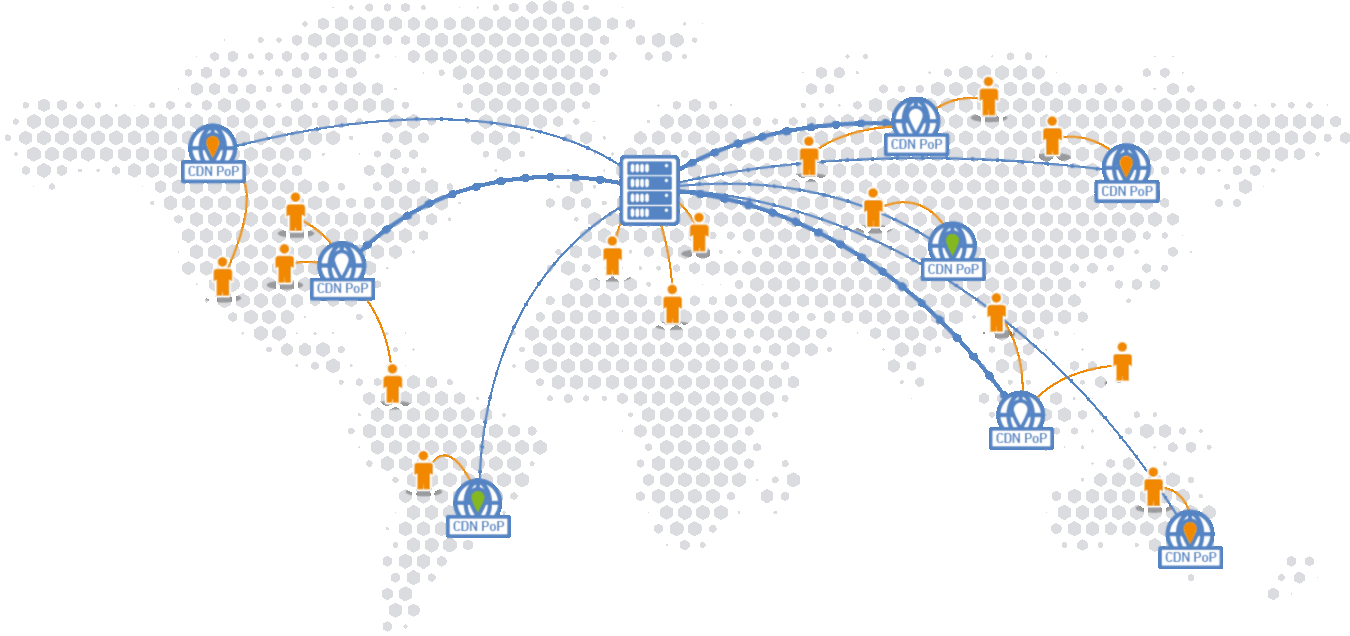
\includegraphics[scale=1]{../images/worldCDN.png}
\end{flushleft}

\bigskip\bigskip\bigskip

\begin{center}
    \itshape{\fontsize{30}{48} \selectfont Pianificazione del Progetto}
\end{center}

\newpage
\printindex

\newpage
\section{\itshape{Pianificazione del Progetto}}
\setlength{\arrayrulewidth}{.5mm}
\setlength{\tabcolsep}{5pt}
\renewcommand{\arraystretch}{2}

\subsection{Introduzione}
Il team seguirà la metodologia di progetto RUP, in seguito sono specificati il piano di progetto e le
iterazioni che lo compongono.

\subsection{Piano}
Il piano di progetto si suddivide in 4 fasi temporali:
\begin{itemize}
    \item Inception
    \item Elaboration
    \item Construction
    \item Transition
\end{itemize}
Le attività coinvolte sono le seguenti:
\begin{itemize}
    \item Studio di fattibilità
    \item Raccolta dei requisiti
    \item Analisi e progetto
    \item Implementazione
    \item Test
\end{itemize}
Le varie attività si distribuiranno nelle fasi temporali in maniera eterogenea, in relazione a quanto una particolare attività è significativa in una certa fase. Qui sotto è raffigurato il processo in un grafico descrittivo: \vspace{0.6cm}

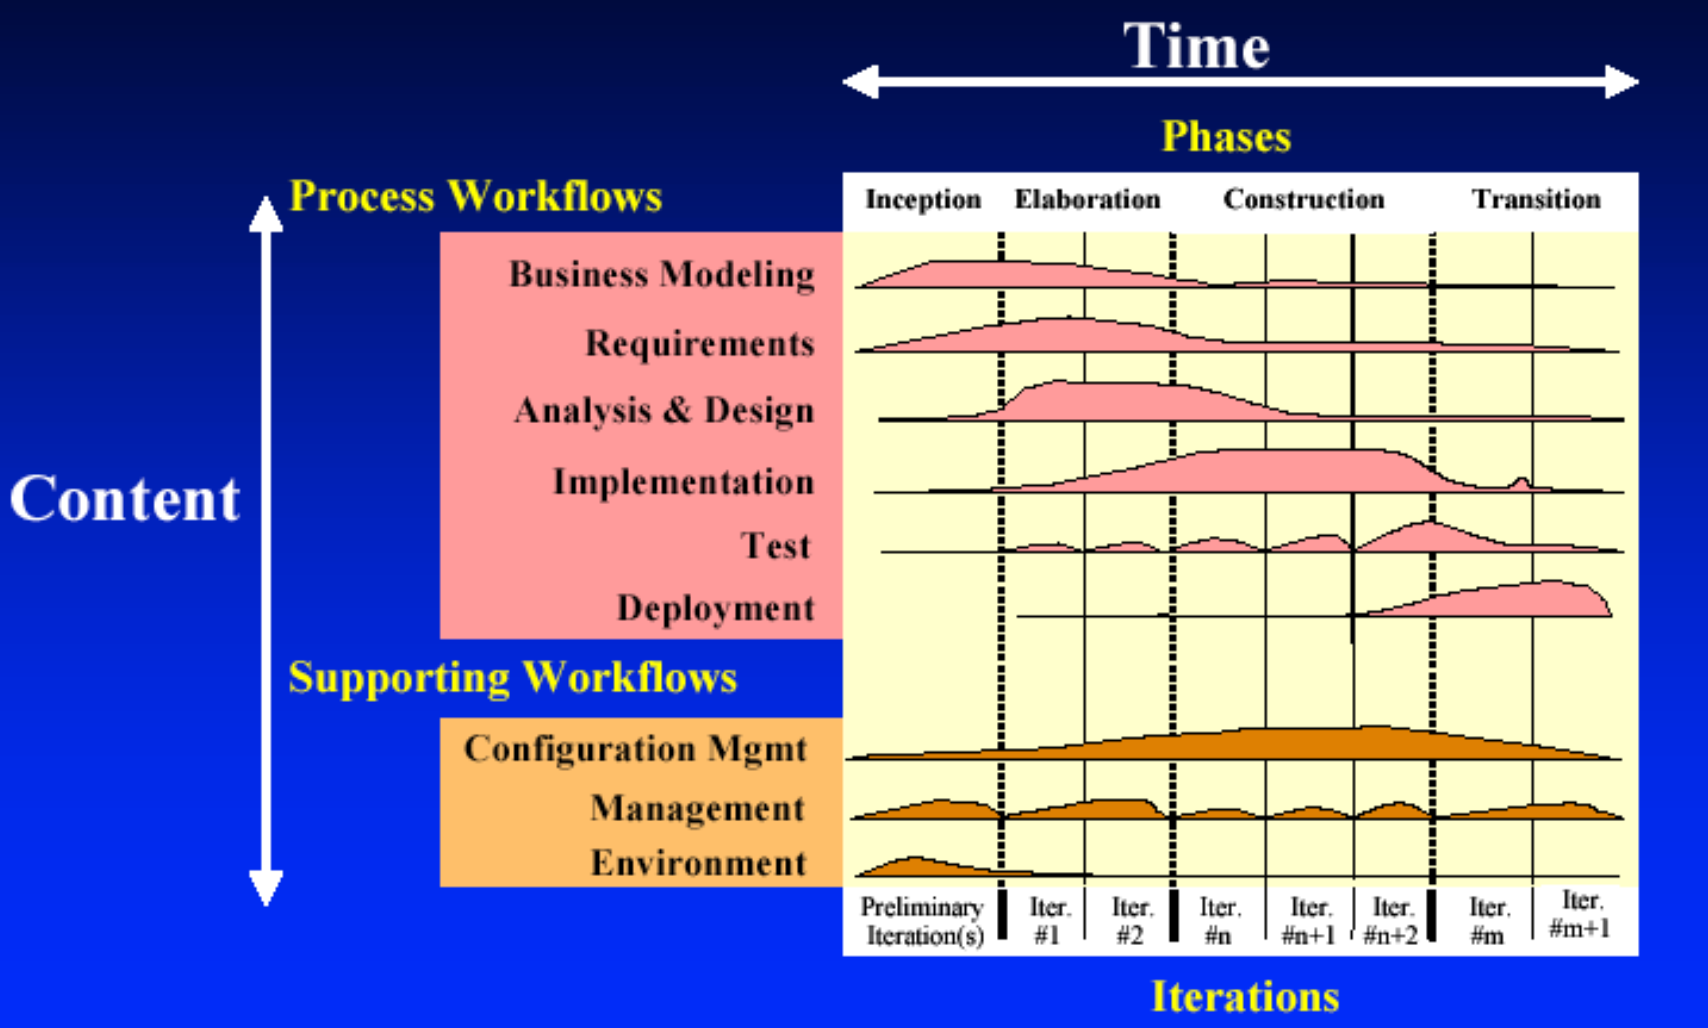
\includegraphics[width=12cm]{RUPplan.png}

\subsection{Iterazioni}

\emph{\textbf{Nota:}} si assume che i requisiti funzionali primari sono tutti quei requisiti con priorità alta e che potrebbero impattare sull'architettura. Al contrario, i requisiti funzionali secondari sono tutti i requisiti con priorità piu bassa e che non hanno impatto sull'architettura.

\begin{center}

\begin{tabular}{ |p{2cm}|p{10cm}|  }
\hline
Nome & Iterazione 1 \\\hline
Fase & Inception \\\hline
Inizio & 20/11/2019 \\\hline
Fine &  1/12/2019 \\\hline
Obbiettivi & 
	\begin{compactitem}
		\item Analisi del problema e prima stesura del documento di Visione
		\item Definire configurazione iniziale del sistema
		\item Analizzare la fattibilità del progetto, dal punto di vista tecnico ed economico
		\item Formulazione di una prima proposta di Contratto
		\item Formulazione documento Glossario
	\end{compactitem}\\\hline
Stato &  Conclusa \\\hline
\end{tabular}
\label{table:1}\newline

\begin{tabular}{ |p{2cm}|p{10cm}|  }
\hline
Nome & Iterazione 2 \\\hline
Fase & Inception \\\hline
Inizio & 15/12/2019 \\\hline
Fine &  18/12/2019 \\\hline
Obbiettivi & 
	\begin{compactitem}
		\item Stesura del piano di progetto
		\item Revisione e aggiornamento della proposta di contratto
		\item Individuare almeno il 50\% dei requisiti funzionali con priorità primaria
	\end{compactitem}\\\hline
Stato &  Conclusa \\\hline
\end{tabular}
\label{table:2}\newline

\begin{tabular}{ |p{2cm}|p{10cm}|  }
\hline
Nome & Iterazione 3 \\\hline
Fase & Inception \\\hline
Inizio & 01/02/2020 \\\hline
Fine &  14/02/2020 \\\hline
Obbiettivi & 
	\begin{compactitem}
		\item Individuare tutti i rimanenti requisiti funzionali con priorità primaria
		\item Individuare almeno il 25\% dei requisiti non funzionali
		\item Descrivere ad alto livello i requisiti individuati
		\item Individuare almeno il 70\% dei rischi e stendere un piano di gestione per ciascun rischio
	\end{compactitem}\\\hline
Stato &  Conclusa \\\hline % Svolgimento 
\end{tabular}
\label{table:3}\newline

\begin{tabular}{ |p{2cm}|p{10cm}|  }
\hline
Nome & Milestone 1\\\hline
Fase & Inception \\\hline
Inizio & 17/02/2020 \\\hline
Fine &  17/02/2020 \\\hline
Obbiettivi & 
	\begin{compactitem}
		\item I requisiti funzionali primari sono stati individuati e descritti correttamente
		\item Almeno il 70\% dei rischi è stato individuato ed è stato creato un piano di gestione per ciascun rischio
		\item Tutte le iterazioni sono state programmate
	\end{compactitem}\\\hline
Stato &  Raggiunta \\\hline
\end{tabular}
\label{table:milestone1}\newline

\begin{tabular}{ |p{2cm}|p{10cm}|  }
\hline
Nome & Iterazione 4 \\\hline
Fase & Elaboration \\\hline
Inizio & 17/02/2020 \\\hline
Fine &  24/02/2020 \\\hline
Obbiettivi & 
	\begin{compactitem}
		\item Iniziare modello di analisi dell'architettura, individuando le classi
		\item Definire il modello dei casi d'uso per il primo 50\% dei requisiti funzionali primari
		\item Individuare 5 requisiti funzionali fondamentali tra i requisiti funzionali primari (che verranno usati per testare l'architettura)
		\item Individuare e descrivere un ulteriore 50\% dei requisiti non funzionali
		\item Individuare un ulteriore 15\% dei rischi e stendere un piano di gestione per ciascun rischio
	\end{compactitem}\\\hline
Stato &  Conclusa \\\hline
\end{tabular}
\label{table:4}\newline

\begin{tabular}{ |p{2cm}|p{10cm}|  }
\hline
Nome & Iterazione 5 \\\hline
Fase & Elaboration \\\hline
Inizio & 26/02/2020 \\\hline
Fine &  03/03/2020  \\\hline
Obbiettivi & 
	\begin{compactitem}
		\item Completare il modello di analisi dell'architettura (completare la descrizione delle classi ed effettuare una suddivisione in package)
		\item Completare il modello dei casi d'uso relativo ai requisiti funzionali primari
		\item Individuare e descrivere i restanti requisiti non funzionali % 100%
		\item Individuare i rischi rimanenti e stendere un piano di gestione per ciascun rischio % 100%
		\item Individuare i primi test sull'architettura e sui requisiti fondamentali
		\item Effettuare una stima dei costi con casi d'uso primari
	\end{compactitem}\\\hline
Stato &  Conclusa \\\hline
\end{tabular}
\label{table:5}\newline

\begin{tabular}{ |p{2cm}|p{10cm}|  }
\hline
Nome & Iterazione 6 \\\hline
Fase & Elaboration \\\hline
Inizio & 05/03/2020 \\\hline
Fine &  14/03/2020  \\\hline
Obbiettivi & 
	\begin{compactitem}		
		\item Iniziare il modello di design dell'architettura
		\item Definire il modello di analisi per i casi d'uso fondamentali individuati
		\item Ampliare i test sull'architettura e sui requisiti fondamentali, in seguito alle scelte di progetto		

	\end{compactitem}\\\hline
Stato &  Programmata \\\hline
\end{tabular}
\label{table:6}\newline

\begin{tabular}{ |p{2cm}|p{10cm}|  }
\hline
Nome & Iterazione 7 \\\hline
Fase & Elaboration \\\hline
Inizio & 15/03/2020 \\\hline
Fine & 25/03/2020 \\\hline
Obbiettivi & 
	\begin{compactitem}
		\item Completare il modello di design dell'architettura
		\item Definire il modello di design per i casi d'uso fondamentali individuati
		\item Implementare l'architettura e i casi d'uso fondamentali individuati
		\item Ultimare i test sull'architettura e sui requisiti fondamentali
	\end{compactitem}\\\hline
Stato &  Programmata \\\hline
\end{tabular}
\label{table:7}\newline

\begin{tabular}{ |p{2cm}|p{10cm}|  }
\hline
Nome & Milestone 2\\\hline
Fase & Elaboration \\\hline
Inizio & 26/03/2020 \\\hline
Fine &  26/03/2020 \\\hline
Obbiettivi & 
	\begin{compactitem}
		\item Tutti i rischi sono stati individuati ed è stato creato un piano di gestione per ciascun rischio
		\item \'E stata effettuata una stima dei costi attendibile
		\item Prendere una decisione Go/NoGo
		\item \'E stata creata una base architetturale coerente con i requisiti ed eseguibile
		\item \'E stato prodotto un modello dei casi d'uso primari sufficientemente dettagliato per iniziare la fase di construction
		\item I casi d'uso fondamentali risultano implementati correttamente con l'architettura prodotta
	\end{compactitem}\\\hline
Stato &  Programmata \\\hline
\end{tabular}
\label{table:milestone2}\newline

\begin{tabular}{ |p{2cm}|p{10cm}|  }
\hline
Nome & Iterazione 8 \\\hline
Fase & Construction \\\hline
Inizio & 27/03/2020 \\\hline
Fine &  04/04/2020  \\\hline
Obbiettivi & 
	\begin{compactitem}

		\item Definire il modello di analisi per il 30\% dei requisiti funzionali primari
		\item Definire il modello di design per il 30\% dei requisiti funzionali primari
		\item Implemetazione e definizione dei test per il 30\% dei requisiti funzionali primari
	\end{compactitem}\\\hline
Stato &  Programmata \\\hline
\end{tabular}
\label{table:8}\newline

\begin{tabular}{ |p{2cm}|p{10cm}|  }
\hline
Nome & Iterazione 9 \\\hline
Fase & Construction \\\hline
Inizio & 05/04/2020 \\\hline
Fine &  12/04/2020  \\\hline
Obbiettivi & 
	\begin{compactitem}
		\item Definire il modello di analisi per un altro 30\% dei requisiti funzionali primari
		\item Definire il modello di design per un altro 30\% dei requisiti funzionali primari
		\item Implementazione e definizione dei test per il 30\% dei requisiti funzionali primari
		
	\end{compactitem}\\\hline
Stato &  Programmata \\\hline
\end{tabular}
\label{table:9}\newline


\begin{tabular}{ |p{2cm}|p{10cm}|  }
\hline
Nome & Iterazione 10 \\\hline
Fase & Construction \\\hline
Inizio & 13/04/2020 \\\hline
Fine &  20/04/2020  \\\hline
Obbiettivi & 
	\begin{compactitem}
		\item Definire il modello di analisi per un altro 30\% dei requisiti funzionali primari
		\item Definire il modello di design per un altro 30\% dei requisiti funzionali primari
		\item Implementazione e definizione dei test per il 30\% dei requisiti funzionali primari
		
		\item individuazione e definizione del modello dei casi d'uso per i requisiti funzionali secondari
	\end{compactitem}\\\hline
Stato &  Programmata \\\hline
\end{tabular}
\label{table:10}\newline

\begin{tabular}{ |p{2cm}|p{10cm}|  }
\hline
Nome & Iterazione 11 \\\hline
Fase & Construction \\\hline
Inizio & 21/04/2020 \\\hline
Fine &  27/04/2020  \\\hline
Obbiettivi & 
	\begin{compactitem}
		\item Definire il modello di analisi per il restante 10\% dei requisiti funzionali primari
		\item Definire il modello di design per il restante 10\% dei requisiti funzionali primari
		\item Implementazione e definizione dei test per il 10\% dei requisiti funzionali primari
		
		\item Definire il modello di analisi dei requisiti funzionali secondari
		\item Definire il modello di design per dei requisiti funzionali secondari
		\item Implementazione e definizione dei test dei requisiti funzionali secondari
		
	\end{compactitem}\\\hline
Stato &  Programmata \\\hline
\end{tabular}
\label{table:11}\newline


\begin{tabular}{ |p{2cm}|p{10cm}|  }
\hline
Nome & Milestone 3\\\hline
Fase & Construction \\\hline
Inizio & 28/04/2020 \\\hline
Fine &  28/04/2020 \\\hline
Obbiettivi & 
	\begin{compactitem}
		\item Sono stati definiti test per ogni funzionalità del sistema
		\item Il sistema e le sue funzionalità implementate hanno superato tutti i test definiti
	\end{compactitem}\\\hline
Stato &  Programmata \\\hline
\end{tabular}
\label{table:milestone3}\newline

\begin{tabular}{ |p{2cm}|p{10cm}|  }
\hline
Nome & Iterazione 12 \\\hline
Fase & Transition \\\hline
Inizio & 29/04/2020 \\\hline
Fine &  2/05/2020  \\\hline
Obbiettivi & 
	\begin{compactitem}
		\item Raccolta Feedback di utilizzo degli utenti
		\item Effettuare correzioni basate sul feedback degli utenti
		\item Creazione degli ultimi test basati sul feedback degli utenti
		\item Creare una release finale
	\end{compactitem}\\\hline
Stato &  Programmata \\\hline
\end{tabular}
\label{table:12}\newline

\begin{tabular}{ |p{2cm}|p{10cm}|  }
\hline
Nome & Milestone 4\\\hline
Fase & Transition \\\hline
Inizio & 03/05/2020 \\\hline
Fine &  03/05/2020 \\\hline
Obbiettivi & 
	\begin{compactitem}
		\item Release finale creata
		\item La release finale supera i test definiti in seguito al feedback degli utenti
	\end{compactitem}\\\hline
Stato &  Programmata \\\hline
\end{tabular}
\label{table:milestone4}\newline


\end{center}

\subsection{Diagramma di Gantt}
\vspace{0.5cm}
\begin{center}
	\hspace*{-2cm}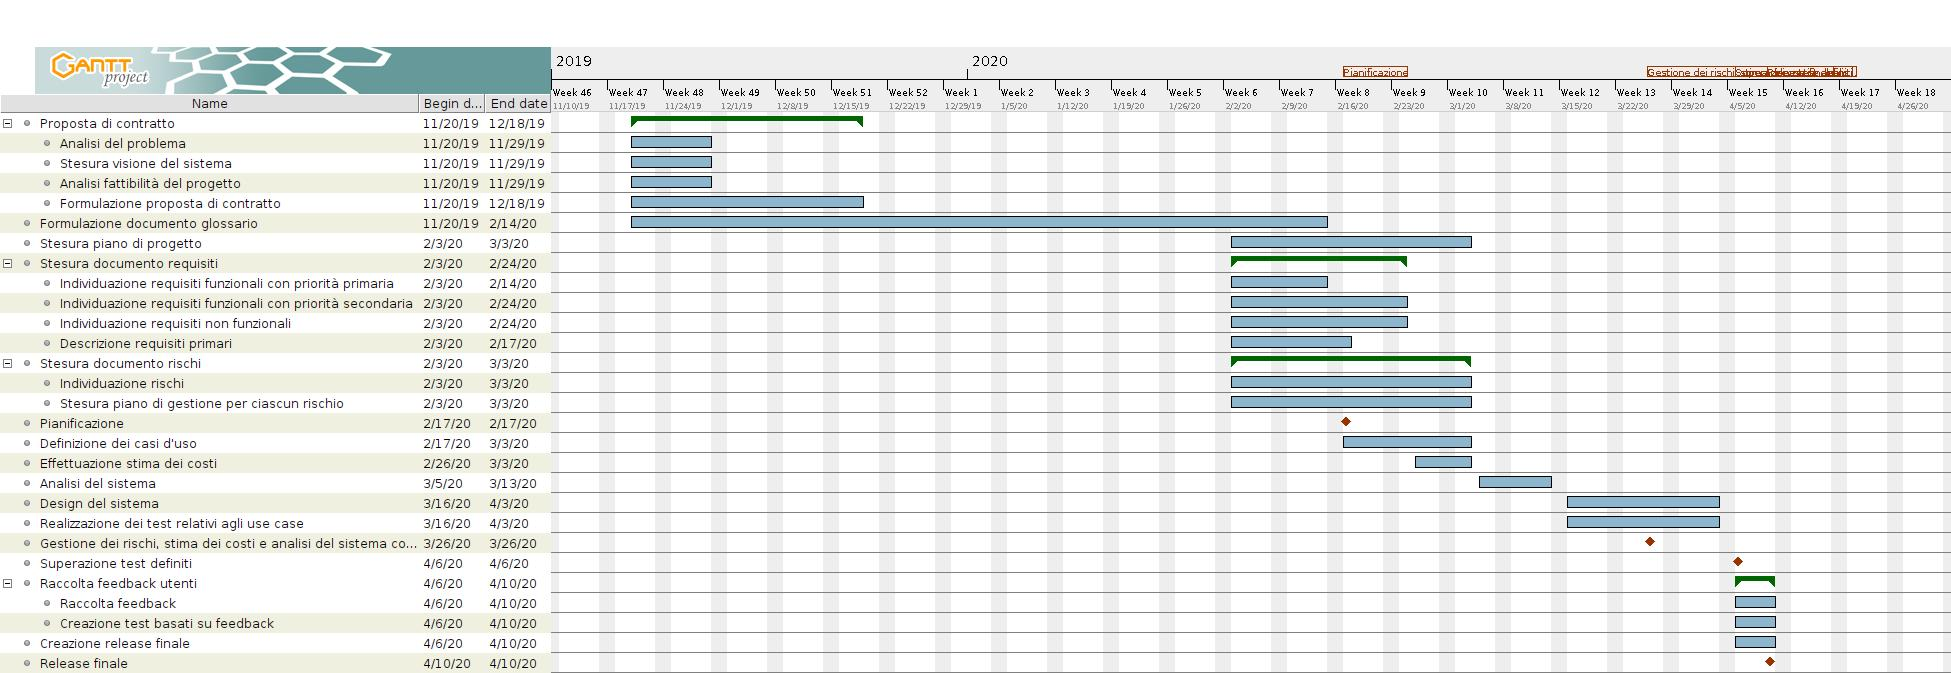
\includegraphics[width=16cm]{Gantt_NexiFy.jpg}
\end{center}
\vspace{2cm}

\clearpage
\noindent{\large \textbf{Revisioni 4-5}} \\ \\
\begin{tabular}{|c | c | c | c|} 
 	\hline
	 Numero & Data & Descrizione \\ [0.5ex] 
	\hline\hline
	1 & 17/12/2019 & Stesura iniziale \\ 
	\hline
	2 & 16/02/2020 & \thead{Specificati meglio gli obiettivi da raggiungere per ogni iterazione,\\e non gli strumenti usati per raggiungerli} \\ 
	\hline
	3 & 26/02/2020 & Revisione del contratto e del piano di progetto \\ 
	\hline
	4 & 14/03/2020 & Specificate meglio attività per implementare l'architettura\\
	\hline
\end{tabular}
\index{Index}

\end{document}
